%%==================================================
%% chapter03.tex for SJTU Master Thesis
%% Encoding: UTF-8
%%==================================================

\chapter{Secure KVM安全嵌套式虚拟化系统的设计与实现}
\label{chap:securekvm}



\section{引言}

随着云计算的不断发展,越来越多的云服务提供商以虚拟主机(Virtual Private Server)的形式为用户提供产品服务。对于用户而言,这种方式带来了无与伦比的灵活性,用户可以自定义虚拟主机上的操作系统、软件栈,就如同拥有一台真实的远程服务器一般。用户甚至可以给云服务提供商直接上传自己的虚拟机镜像,其应用程序便可以直接在云平台上运行,大大简化了部署的过程。对于云服务提供商而言,目前有丰富的开源虚拟化平台可供采用,通过将多台客户虚拟主机整合到单台物理机器上运行,其可以提高资源利用率,减少在硬件投入和能源消耗上的成本。总而言之,多租户云的普及,这是一个双赢的过程。

可是,事物总有其双面性,如何保障客户虚拟主机中敏感数据的安全性和私密性,是在多租户云环境中必须面对的一个突出问题。用户在虚拟主机中往往会保存一些敏感数据,如用于非对称加密的公私钥、存储用户名密码的数据库表等,由于现有虚拟化平台的局限性,这些敏感数据均能很容易地被恶意虚拟机监控器或者云服务提供商操作人员窥测到,存在泄漏的风险。

在本章中,我们借助嵌套式虚拟化,提出了一种透明、向前兼容的增强客户虚拟机中敏感数据安全的解决方案。通过在现有虚拟机监控器下方加入嵌套式虚拟化层,我们可以监控虚拟机监控器的行为,避免其对客户虚拟机的内存、磁盘数据安全造成威胁。Secure KVM以可接受的性能开销作为代价,保障了客户虚拟机中敏感数据的安全性与隐私性。

\section{背景介绍及问题分析}

\subsection{虚拟化本质论}

所谓“系统虚拟化”,亦即VMM虚拟机监控器给客户操作系统和应用程序提供一个虚拟的运行平台,而这个虚拟运行平台要与真实硬件基本无异,不能让客户操作系统和应用程序感受到差别(现阶段,打通VMM虚拟机监控器和Guest VM客户虚拟机之间的语义隔阂,主动让客户虚拟机意识到自己运行在虚拟化平台上以获得性能提升的情形也是存在的,在本文中我们忽略这样的特例)。

对于一个虚拟的运行平台而言,有三个主要组成要素,分别是CPU、内存和外设(磁盘和网卡属于此类)。关于CPU,虚拟机监控器要将物理机器上的计算资源即CPU时间片分一部分给客户虚拟机,同时又必须保证CPU资源不能被某一客户虚拟机长期无节制地占用,以免耽误虚拟机监控器自身和其他客户虚拟机的正常运行(类似于操作系统和应用程序之间的关系)。对于内存,虚拟机监控器同样要在满足客户虚拟机内存资源分配的同时保证安全,即某一客户虚拟机必须有节制地使用内存,该客户虚拟机和虚拟机监控器、该客户虚拟机和其他客户虚拟机之间必须保证内存隔离。对于外设,虚拟机监控器要对他们的IO行为进行精确模拟,这一般是通过截获IO指令和MMIO读写操作来完成。

这所有的一些,均要求虚拟机监控器处在比客户虚拟机更高的运行级别。对于CPU,虚拟机监控器要在某一客户虚拟机时间片用完时(时间中断到来),立即获得执行机会抢占该客户虚拟机,并切换另一客户虚拟机上来运行。对于内存,虚拟机监控器要通过一些类似页表的硬件机制限制客户虚拟机的访存范围。对于截获IO指令和MMIO读写,这同样需要高运行级别和硬件机制来保证。

具体到x86硬件虚拟化,虚拟机监控器处在高权限级别的根模式(root mode),客户虚拟机处在低权限级别的非根模式(non-root mode)。当客户虚拟机处在非根模式运行期间发生时间中断时,处理器会以外部中断(External Interrupt)到来的原因陷入到根模式,让虚拟机监控器处理。2007之后Intel推出的第二代硬件虚拟化处理器,均支持扩展页表(Extended Page Table,简称EPT),可以在硬件层面上限制客户虚拟机的内存访问。最后,虚拟机监控器可以指定IO位图,让非根模式下期望的IO指令发生陷入(MMIO读写与此基本类似),并对其进行指令模拟以达到模拟真实设备行为的目的。

不可否认,为了达到系统虚拟化的目的,在一般情况下让虚拟机监控器处在高权限级别是一个必要条件。但与此同时带来的是,虚拟机监控器不受管控的“为所欲为”,给客户虚拟机运行的安全性和隐私性带来了重大隐患。此情形在多租户云、第三方虚拟机提供商等应用环境下体现得尤为明显。下面两节分别从内存和磁盘的角度对此进行详细阐述。

\subsection{客户虚拟机的内存安全}

客户虚拟机的内存中包含有其正在运行程序的所有信息,包括操作系统层面的进程信息、模块信息和应用程序地址空间中的所有数据、代码区域。举例来说,客户虚拟机中的浏览器打开了网银的登录界面而用户正在输入其账号密码,这些隐私数据都是会被保存到客户虚拟机的内存中。

扩展页表限制的是客户虚拟机的访存范围,而虚拟机监控器处在最高权限级别,其可以将物理上的任意内存区块映射到自己的地址空间,并进行访问改写。同样以上文用户网银登陆为例,恶意虚拟机监控器在得知这一信息后,可以对整个客户虚拟机的内存空间进行转储(dump),并在事后进行查找分析,导致用户的敏感隐私数据极有可能因此而被暴露偷窥。

尽管恶意虚拟机监控器起先获取的可能只是庞杂的原始字节数据,其可以利用特殊寄存器数据、特定操作系统内存地址空间结构等信息作为提示,借助虚拟机自省(Virtual Machine Introspection,VMI)等技术手段,从中萃取出隐私数据和语义信息,毕竟这在理论上是可能的。

\subsection{客户虚拟机的磁盘安全}

在真实机器上读磁盘的过程可以简化为此,操作系统先在内存中预留一段区域,然后将待读取数据在磁盘上的位置和预留内存地址等信息通过IO指令告诉磁盘,磁盘通过直接内存访问(Direct Memory Access,DMA)将数据填写到预留内存区域,最后发送中断告诉操作系统数据已经准备就绪。写磁盘的过程基本与此类似。在虚拟化环境下,虚拟机监控器模拟了上述DMA的过程,其在根模式截获敏感IO指令,从磁盘映像中获取对应数据并填至客户虚拟机内存,最后注入虚拟中断告知完成。可以看到,虚拟机监控器处在客户虚拟机的IO数据路径之中,其可以对磁盘IO数据进行任意偷窥甚至修改,威胁客户虚拟机的磁盘安全。

此外,客户虚拟机的磁盘映像直接以明文形式保存在虚拟机监控器中,恶意虚拟机监控器可以在挂载该磁盘映像后对其中文件系统进行任意查看和改动,以更直接的方式对客户虚拟机的磁盘安全造成威胁。



\section{Secure KVM系统的设计}

\subsection{嵌套式虚拟化}

如果虚拟机监控器仍处于系统中的最高权限运行级别,那么能对其进行行为监控的只有处于
更低级别的处理器硬件了,这在目前的角度来看显然是不实际的。因此为了达到目的,我们
只能降低原虚拟机监控器的运行级别(即将其从根模式移出至非根模式),而让我们用于监
控虚拟机监控器行为的可信代码在最高权限级别根模式运行。这样,有了处理器硬件上不同
权限级别的保证,原虚拟机监控器中所进行的一切敏感操作都能被可信监控代码截获并进行
检查,从而保证客户虚拟机的运行安全,此即为安全嵌套虚拟化的主要思想。

\begin{figure}[!htp]
  \centering
  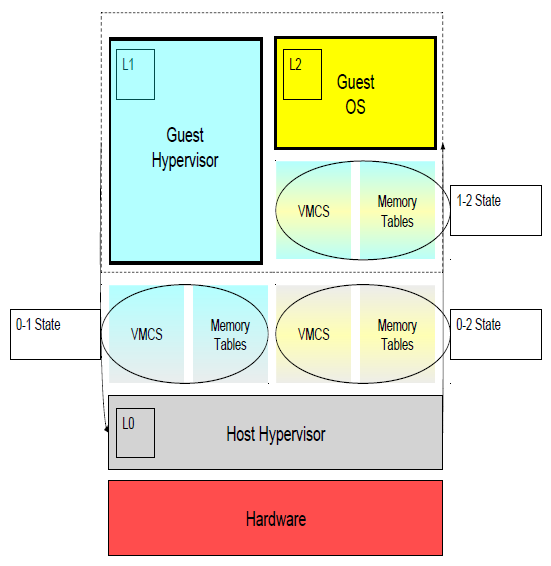
\includegraphics[width=0.7\textwidth]{chap3/nested.png}
  \bicaption[fig:nested]{嵌套式虚拟化示意图}{嵌套式虚拟化示意图}{Fig}{Illustration on nested virtualization}
\end{figure}

图\ref{fig:nested}展示了典型嵌套式虚拟化平台的主体结构,其中主要包含了L0、L1和L2三个层次。

\begin{itemize}
\item{L0(Host hypervisor):嵌套式虚拟化层,处于根模式运行。L1和L2中发生VMExit后均会陷入至此。}
\item{L1(Guest hypervisor):即为原虚拟机监控器,处于非根模式运行。为L2提供运行虚拟化支撑的同时受到L0的管控。}
\item{L2(Guest VM):即为原客户虚拟机,处于非根模式运行。用户应用程序在此运行。}
\end{itemize}

x86处理器硬件上主要有两个结构对非根模式下的运行进行控制,分别是VMCS(Virtual Machine Control Structure)和EPT。嵌套式虚拟化层L0为了支撑原虚拟机监控器L1的运行,为其准备了VMCS和EPT,我们将这一部分状态定义为“0-1状态”。原虚拟机监控器L1为了支撑原客户虚拟机L2的运行,同样为其准备了VMCS和EPT,我们将这一部分状态定义为“1-2状态”。然而,x86处理器没有从硬件上直接支持多层嵌套虚拟化(只有根模式和非根模式两种运行权限级别),也就是说实际上L1和L2处在同样的权限级别均在L0的管控下直接运行,因此L0需要为L2的运行提供额外的VMCS和EPT(相当于0-1状态和1-2状态的合并),我们将其定义为“0-2状态”。下文说明了嵌套式虚拟化系统运行的一个典型流程。

\begin{enumerate}
\item L0以VMCS0-1运行L1
\item L1准备VMCS1-2并执行vmlaunch/vmresume启动L2
\item vmlaunch产生陷入至L0,执行流由L0接管
\item L0将VMCS0-1和VMCS1-2合并,生成VMCS0-2
\item L0以VMCS0-2运行L2
\item L2在非根模式下运行,一段时间后产生陷入
\item 执行流再次由L0接管,L0根据VMExit类型选择自己处理或传递给L1处理
\item 如果L0自己能处理陷入,则vmresume继续执行L2。如果必须交给L1处理,L0根据VMCS0-2准备VMCS0-1和VMCS1-2,并将执行流切换到L1
\item 在1\~~8或5\~~8之间重复
\end{enumerate}

\subsection{系统总体架构}





\section{对客户虚拟机内存的安全保护}



\subsection{基本原理}

\subsection{特殊边界情形处理}




\section{对客户虚拟机磁盘数据的安全保护}

\subsection{基本原理}

在正常的磁盘虚拟化过程中,磁盘读取即是虚拟机监控器将被请求的磁盘数据块从磁盘映像中取出并放置到客户虚拟机指定的内存位置。反之,磁盘写入则是虚拟机监控器从客户虚拟机指定内存位置获取待写数据并存储到磁盘映像相应位置。

由于L2客户虚拟机的设备IO部分仍由L1虚拟机监控器来模拟,L1负责L2实际磁盘IO数据的读取和保存,L2的RAW磁盘映像亦被存储在L1,完全绕过L1不让其接触L2的磁盘IO数据是不实际的。而我们又要保护L2磁盘IO的安全性,故只能退而求其次,让L1始终只能接触到L2加密后的磁盘IO数据。在加密密钥没有被泄露给L1的前提下,加过密的磁盘IO数据对于L1是没有意义的。

要做到这一点,以下四个条件必须得到满足:

\begin{itemize}
\item{L1中存储的L2客户虚拟机磁盘映像必须事先经过加密。否则,L1可以直接以静态方式挂载访问L2磁盘分区和文件系统中的内容。}
\item{当L2进行磁盘读取时,加密后的L2磁盘数据必须要在L1将其读取到相应L2内存空间之后和L2实际使用这一部分数据之前,得到解密。且解密后的这部分数据存在的L2内存空间,L1是被禁止访问的。}
\item{当L2进行磁盘写入时,原先的明文L2待写磁盘数据必须要在L1能接触到其并将其写入磁盘映像之前,得到加密。也就是说,待写磁盘数据在被加密前,其所存在的L2内存空间,L1是被禁止访问的。}
\item{以上三个条件必须做到对L2完全透明,对L1基本透明(L1其实可以发现其上保存的L2磁盘映像是经过加密的)。}
\end{itemize}

对于第一个条件,我们可以用现有的成熟加解密方案处理L2磁盘映像,如AES和DES。

对于第二和第三个条件,L0可以为之完成相应的加解密工作,也可以限制L1对L2的访存范围(通过上节论述)。这里隐含的一个条件是,L0必须能够及时地获取执行机会,也就是说,在需要L0进行加解密时L0必须要得到及时通知。万幸的是,L2客户虚拟机在进行磁盘读取和写入时,均包含了一些敏感操作(IO指令或读写MMIO地址),会立即产生到L0的虚拟机陷入(VMExit),从而让L0得到通知。

对于第四个条件,L2始终接触到的均是明文数据,其不会觉察到L0和L1在事关其磁盘数据安全上做出的斗争。对于L1,除了观察到磁盘映像经过加密这一事实外,在其不威胁L2磁盘数据安全的前提下,其所经历的行为也和正常磁盘虚拟化过程无二致。


\subsection{PIO读部分的处理}

在L2客户操作系统刚启动时,其通过PIO(Programmed Input/Output)的方式读取磁盘数据。PIO是一种同步的简单磁盘数据访问方式。x86处理器上有256个IO端口,其中的一部分被预留给了IDE控制器,如下表所示。而处理器通过x86 ISA中的IO指令(in、out、ins、outs)来读写这些IO端口,来达到访问磁盘数据的目的。PIO的过程是同步的,处理器在执行这些IO指令时不能进行其他工作。待真正进行数据读取的ins(或带req指令前缀的ins指令)执行结束后,磁盘数据即存在于内存中的对应地址。

\begin{table}[htpb]
\bicaption[tab:pio]{磁盘PIO对IO端口的使用说明表}{磁盘PIO对IO端口的使用说明表}{Table}{x86 IO port used in disk PIO}
\centering
\resizebox{\textwidth}{!}{
\begin{tabular}{ccc}
\toprule
Port Offset	& Function & Description\\
\midrule
0	& Data Port	& Read/Write PIO data bytes on this port.\\
1	& Features / Error Information	& Usually used for ATAPI devices.\\
2	& Sector Count	& Number of sectors to read/write (0 is a special value).\\
3	& Sector Number / LBAlo	& This is CHS / LBA28 / LBA48 specific.\\
4	& Cylinder Low / LBAmid	& Partial Disk Sector address.\\
5	& Cylinder High / LBAhi	& Partial Disk Sector address.\\
6	& Drive / Head Port	& Used to select a drive and/or head. May supports extra address/flag bits.\\
7	& Command port / Regular Status port	& Used to send commands or read the current status.\\
\bottomrule
\end{tabular}
}
\end{table}

以下是一个典型的PIO读数据过程。L2先进行IDE主盘/从盘选择,并将之与扇区逻辑块地址(LBA,Logical Block Addressing)高4位作或运算,写入0x1F6端口。随后,L2向0x1F1中写入一个零字节,向0x1F2中写入待读取扇区的数量,并把剩余的LBA地址部分分段写入至0x1F3\~0x1F5。待地址和长度信息写入完毕后,L2向命令端口0x1F7发出读数据指示并轮询等待设备就绪,最后执行rep ins指令接收磁盘数据。

\begin{enumerate}
\item Send 0xE0 for the ``master'' or 0xF0 for the ``slave'', ORed with the highest 4 bits of the LBA to port 0x1F6: outb(0x1F6, 0xE0 | (slavebit << 4) | ((LBA >> 24) & 0x0F))
\item Send a NULL byte to port 0x1F1, if you like (it is ignored and wastes lots of CPU time): outb(0x1F1, 0x00)
\item Send the sectorcount to port 0x1F2: outb(0x1F2, (unsigned char) count)
\item Send the low 8 bits of the LBA to port 0x1F3: outb(0x1F3, (unsigned char) LBA))
\item Send the next 8 bits of the LBA to port 0x1F4: outb(0x1F4, (unsigned char)(LBA >> 8))
\item Send the next 8 bits of the LBA to port 0x1F5: outb(0x1F5, (unsigned char)(LBA >> 16))
\item Send the ``READ SECTORS'' command (0x20) to port 0x1F7: outb(0x1F7, 0x20)
\item Wait for an IRQ or poll.
\item Transfer 256 words, a word at a time, into your buffer from I/O port 0x1F0. (In assembler, REP INSW works well for this.)
\item Then loop back to waiting for the next IRQ (or poll again -- see next note) for each successive sector.
\end{enumerate}

在非嵌套式虚拟化环境下,每条IO指令均会引发VMExit,最终执行流会转移至Qemu并由其对这些IO指令进行模拟。Qemu对除最后一条rep ins指令外的其他IO指令,均只做简单的簿记工作。到了最后的rep ins指令时,Qemu会根据之前记录的扇区地址和数量信息,从磁盘映像对应位置用pread读出数据并写入虚拟机内存空间对应位置,最后Qemu会调整虚拟机指令指针寄存器rip的数值以恢复虚拟机从下一条指令执行。

由于存放在L1原虚拟机监控器中的L2磁盘映像是经过加密的,L1向L2内存空间中写入的PIO磁盘数据便也是以密文形式存在。为了让L2客户虚拟机正常运行,我们必须适时地对密文PIO磁盘数据进行解密。这个数据解密的时机,便在L1向L2内存空间写入数据后正要恢复L2执行时。这时,待读取磁盘数据已经完整存在于L2内存空间而L2还未能访问这部分数据,且L1用来恢复L2执行的vmresume指令会产生到L0嵌套式虚拟化层的陷入。此过程用UML顺序图可以表示如下。

\begin{figure}[!htbp]
  \centering
  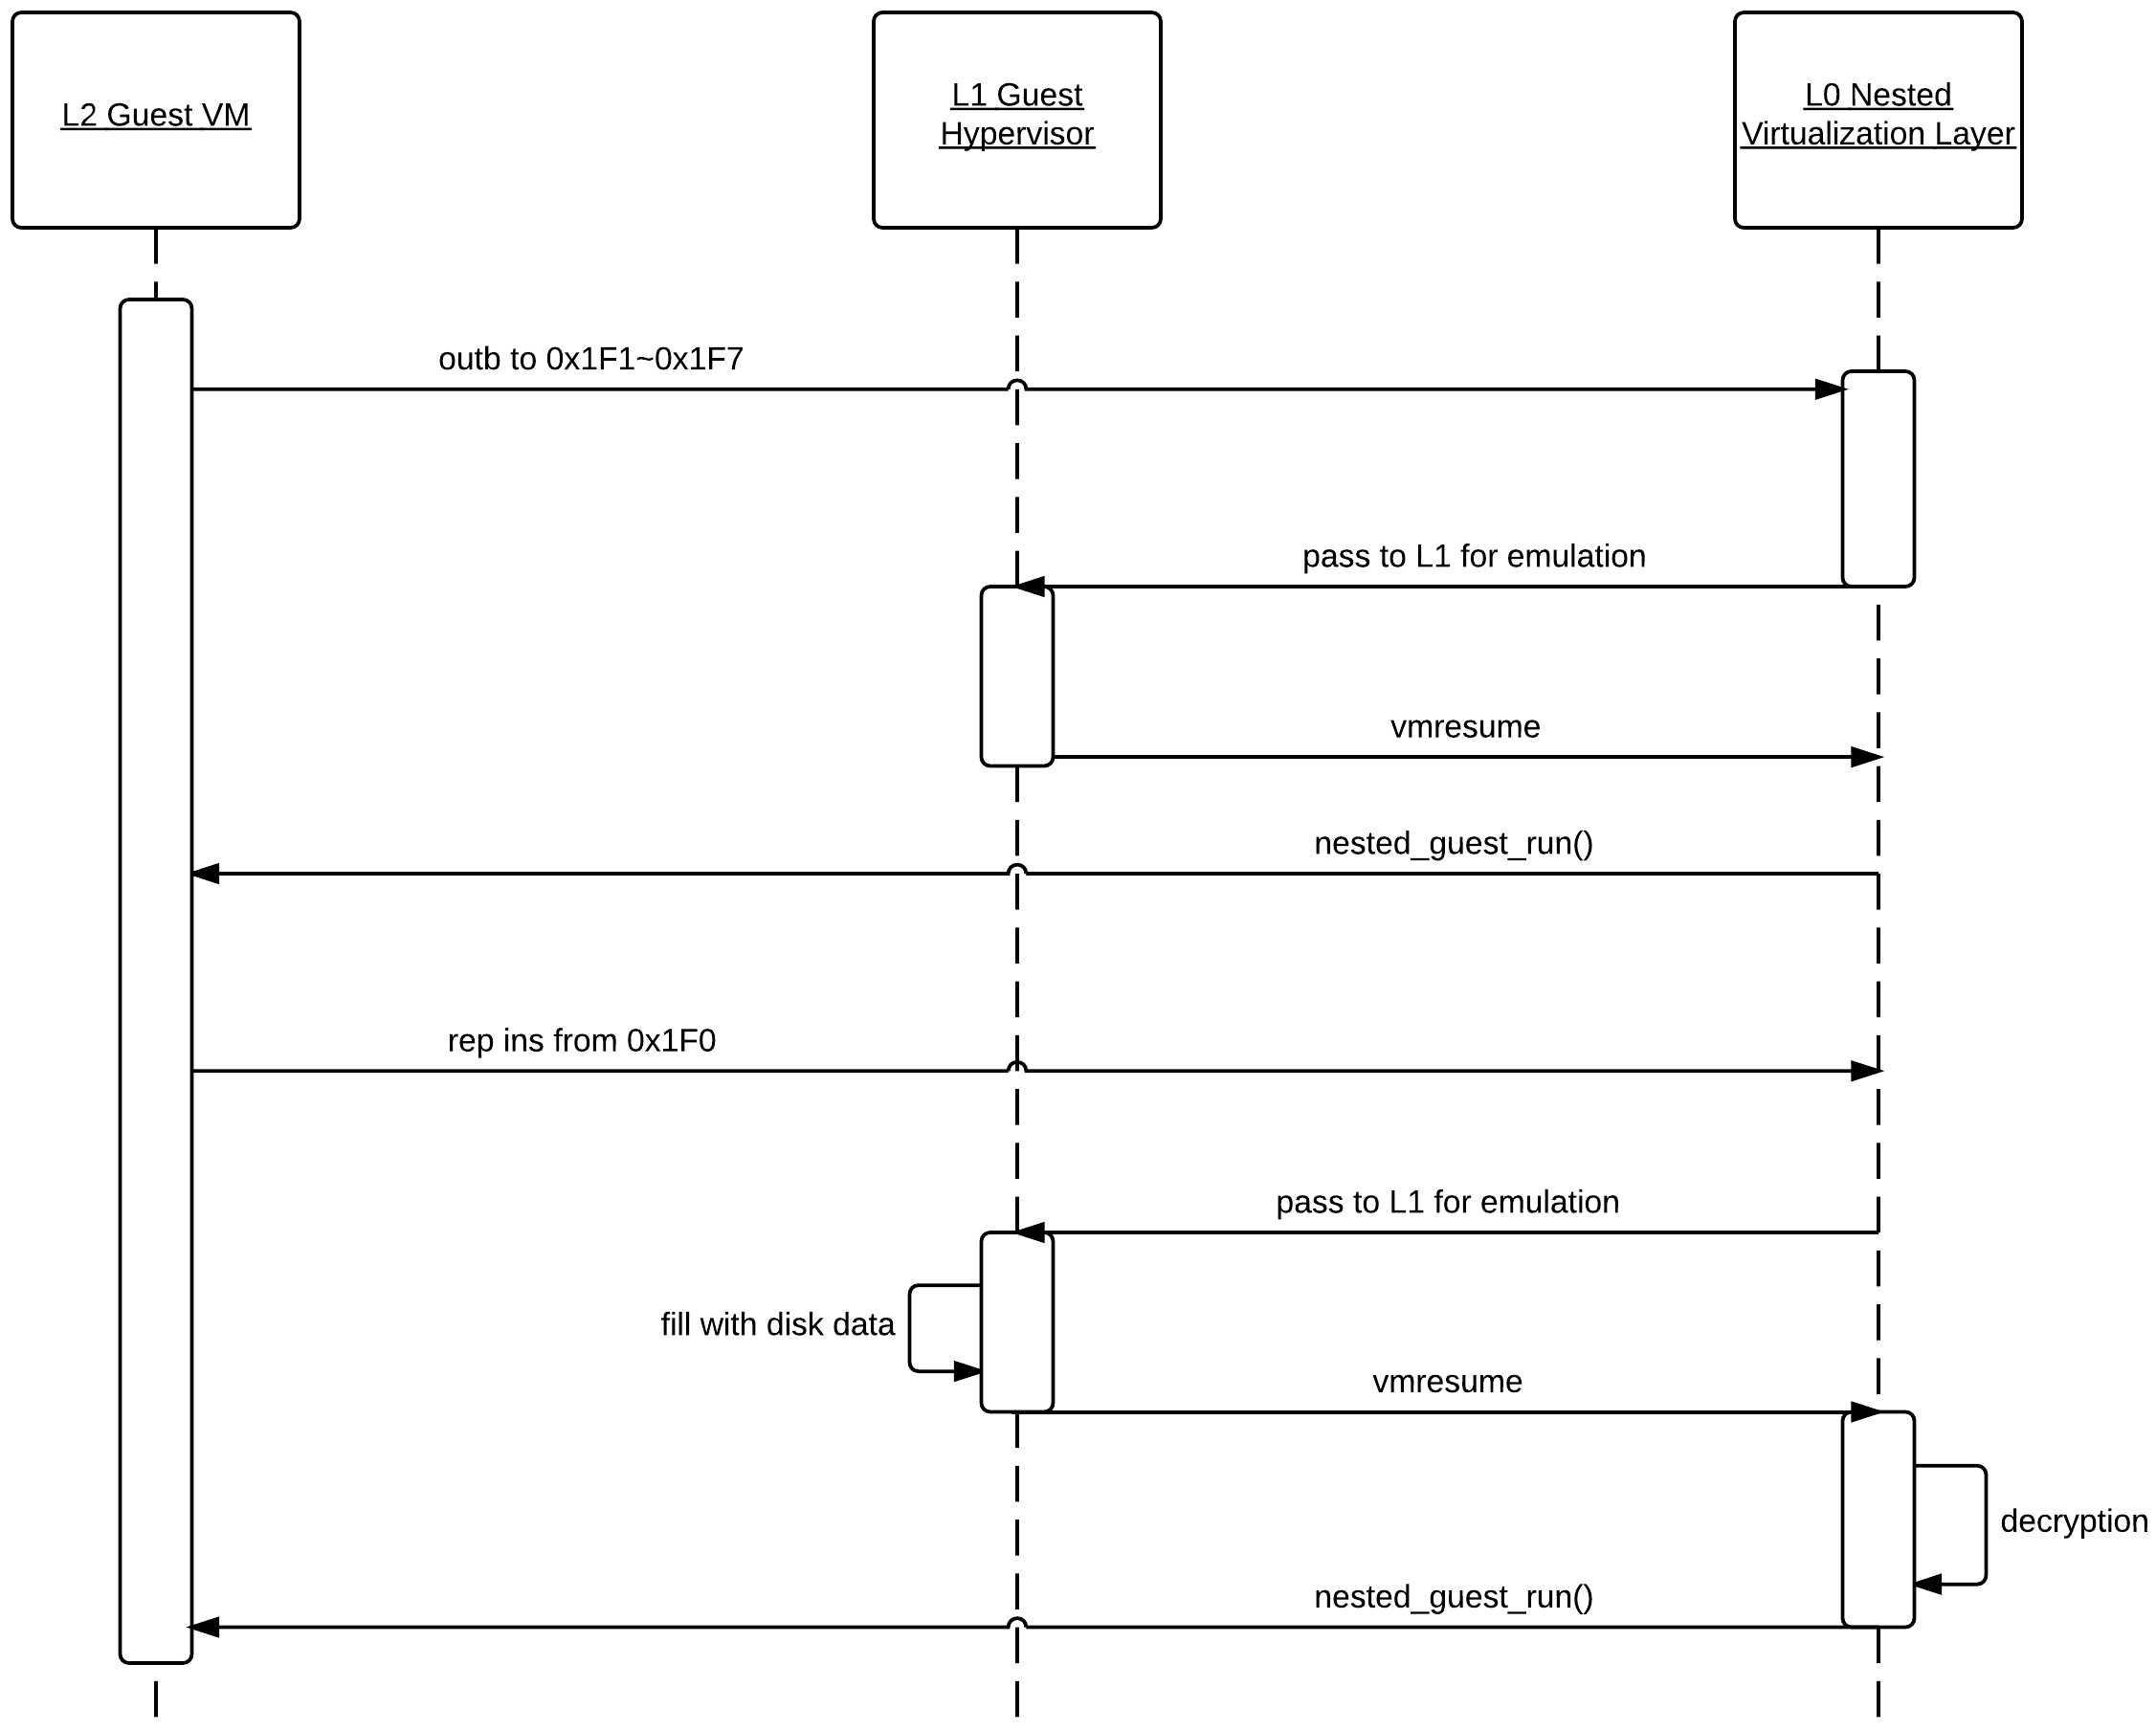
\includegraphics[width=0.7\textwidth]{chap3/pio_read.png}
  \bicaption[fig:pio_read]{嵌套式虚拟化示意图}{嵌套式虚拟化示意图}{Fig}{Illustration on nested virtualization}
\end{figure}

L2客户虚拟机进行PIO磁盘读取的粒度是8个磁盘扇区,即每次读取连续的8个普通磁盘扇区,正好是一个对齐的内存页(512B * 8 = 4KB)。L0对其进行解密的过程即为将对应的存放加密磁盘数据的内存页面映射到自己的地址空间,然后用事先约定好的密钥在原地址进行解密操作,其中所涉及到的多层内存地址转换、加解密算法等细节问题将在接下来的章节中进行详细论述。

此外,在原型系统的开发过程中,于PIO层面,我们仅发现有读取行为而未发现磁盘写入。我们猜测PIO读取仅用于Linux初期启动过程中grub将操作系统内核等必要数据载入客户虚拟机内存,待到Linux启动完成后,所有的磁盘操作将转由效率更高的DMA来进行,这部分的论述将在接下来的两节中完成。

\subsection{DMA读部分的处理}

在L2客户虚拟机操作系统加载并初始化完毕后,通过PIO从磁盘读取数据的方式便不再被使用,此时的磁盘操作将转由DMA方式进行。DMA读是一个异步的过程,处理器先将待读取磁盘扇区的信息用IO指令的方式通知IDE控制器(此部分数据的传输与PIO类似),随后再传输描述存放待读取数据缓冲区内存地址的数据结构并发出DMA指令。IDE控制器收到指令后,利用系统总线的空闲期在后台传输读取到的磁盘数据并写入内存缓冲区,在此过程中无需处理器的参与,处理器在此阶段可以继续执行其他指令。等到数据传输完毕后,IDE控制器再向处理器发送特定中断,通知其数据读取已经完成。

描述存放待读取数据缓冲区内存地址的数据结构被称作物理区域描述符表(Physical Region Descriptors Table,PRDT)。PRDT中的每个表项大小为8个字节,0-3字节说明内存页面的物理地址,4-7字节说明内存区域的大小,以字节为单位,全零表示64K字节。PRDT表最后一个表项第7字节的最高一位如果被置上则表示PRDT表的结束。之所以要使用PRDT表作为描述内存缓冲区的数据结构,是因为很难从低端内存中找到物理上连续的大块区域(只有低端内存,即物理地址低于32MB的内存空间,能被一般DMA设备访问)。PRDT表实际上是从逻辑角度将多块较小的物理上不连续的内存区域拼凑出了一块虚拟的大块内存区域,类似于集散序列(scatter-gather list)。

以下是一个典型的DMA读数据过程。

\begin{enumerate}
\item 软件准备好一个PRD Table放在内存中,每个8字节,对齐到4字节边界。

\item 软件把PRD table的起始地址设置好,同时通过设置读/写控制位设置数据和传输方向,清除状态寄存器中的中断位和错误位。

\item 软件发出DMA传送指令到disk设备。

\item 向总线控制器IDE命令寄存器的对应通道中写入1,使能总线控制器。

\item DMA从IDE设备中请求控制器传送数据到/从内存中

\item 传送结束,IDE设备发出中断

\item 接收到中断后,软件设置命令寄存器的开始/结束位,然后先后读控制器状态、驱动状态,进而确定是否传送成功。
\end{enumerate}

TODO:PCI 中断识别

\subsection{DMA写部分的处理}

TODO: Tranpoline Buffer

\subsection{多层内存地址转换的处理}

在嵌套式虚拟化环境下,各层内存地址之间的转化关系尤为复杂,其中经常涉及到的内存地址有以下几种。

\begin{enumerate}
\item L2 GVA,即L2 Guest Virtual Address,L2客户虚拟机中的线性虚拟地址,L2中的应用程序和操作系统内核使用此地址访问内存
\item L2 GPA,即L2 Guest Physical Address,L2客户虚拟机中的物理地址,可以由L2 GVA通过页表转换得到
\item L1 GPA,即L1 Guest Physical Address,L1虚拟机监控器中的物理地址
\item L0 HVA,即L0 Host Virtual Address,L0嵌套式虚拟化层中的线性虚拟地址,L0通过此地址来访问机器上所有的内存空间
\item L0 HPA,即L0 Host Physical Address,L0嵌套式虚拟化层中的物理地址或机器地址,可以由L0 GVA通过页表转换得到
\end{enumerate}

在如此多种内存地址中间,又有若干种页表(或辅助扩展页表)来控制它们之间的转换关系,如图\ref{fig:paging}所示。

\begin{enumerate}
\item L2 PT,负责L2 GVA到L2 GPA的转换,由L2负责维护
\item L1 EPT12,负责L2 GPA到L1 GPA的转换,由L1负责维护
\item L0 EPT01,负责L1 GPA到L0 HPA的转换,由L0负责维护
\item L0 EPT02,负责L2 GPA到L0 HPA的转换,由L0负责维护
\item L0 PT,负责L0 HVA到L0 HPA的转换,由L0负责维护
\end{enumerate}

从逻辑上来说,L2客户虚拟机运行时存在着三层地址转换关系,L2 GVA到L2 GPA的转换,L2 GPA到L1 GPA的转换,和L1 GPA到L0 HPA的转换。但是,CPU在硬件上仅仅支持两层地址转换关系,即普通页表和辅助扩展页表。因此,L0嵌套式虚拟化层需要对后面两层地址转换关系进行压缩合并,在L2客户虚拟机运行时CPU实际使用的辅助扩展页表是EPT02。

\begin{figure}[!htbp]
  \centering
  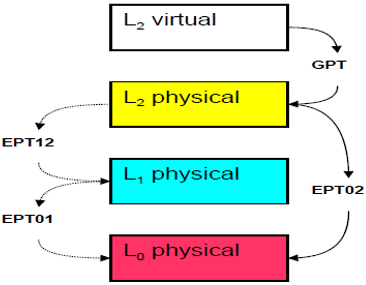
\includegraphics[width=0.7\textwidth]{chap3/paging.png}
  \bicaption[fig:paging]{多层内存地址转换示意图}{多层内存地址转换示意图}{Fig}{Illustration on Multi-dimensional Paging}
\end{figure}

在L0嵌套式虚拟化层进行磁盘数据加解密时,必须适时地进行内存地址之间的转换。如负责L2 GPA到L1 GPA转换的EPT12表,其根地址和表项中的地址数据均以L1 GPA的形式存在。又如L2客户虚拟机进行DMA操作时使用的PRDT表,其中的表项地址数据以L2 GPA的形式存在。下文将以L2 GPA到L0 HVA为例,详述其中的地址转换过程。

L0先去EPT02中查找L2 GPA到L0 HPA的对应关系,此功能由ept02\_p2m函数实现。ept02\_p2m先从当前VMCS中读出EPT02表的根地址,然后模拟硬件查表行为,将L2 GPA划分为4段并分别去索引EPT表的每一级。如EPT02表中每一级表项都存在且合法,ept02\_p2m将返回转换后的L0 HPA,否则ept02\_p2m将返回0表示此次尝试失败。

\begin{lstlisting}[language={C}, caption={ept02\_p2m实现源代码}]
static unsigned long ept02_p2m(unsigned long pfn) {
    unsigned long ept_hpa = vmcs_readl(EPT_POINTER);
    int l4i, l3i, l2i, l1i;
    unsigned long mfn;
    ept_entry_t *ept_hvm, *cur_epte, *l2_epte;

    ept_hvm = (ept_entry_t*)pfn_to_kaddr(ept_hpa >> PAGE_SHIFT);

    l4i = (pfn >> 27) & 0x1ff;
    l3i = (pfn >> 18) & 0x1ff;
    l2i = (pfn >> 9) & 0x1ff;
    l1i = pfn & 0x1ff;

    /* L4 */
    cur_epte = ept_hvm + l4i;
    if (!(cur_epte->epte & 0x7)) {
        return 0;
    }
    
    /* L3 */
    cur_epte = (ept_entry_t*)(pfn_to_kaddr(cur_epte->mfn)) + l3i;
    if (!(cur_epte->epte & 0x7)) {
        return 0;
    }
    if (cur_epte->sp_avail) {
    	/* 1G super page */
        mfn = cur_epte->mfn + (pfn & 0x3ffff);
        return mfn;
    }

    /* L2 */
    ......
    /* L1 */
    ......

    mfn = cur_epte->mfn;
    return mfn;
}
\end{lstlisting}

但是在KVM中,为了节省内存开销,EPT表采用按需填充(populate on demand)的方式进行更新,即EPT在客户虚拟机刚启动时仅为一张空表,其中内容只有等到页错误发生时才会被增添或修改。这个特性会给内存地址转换带来问题,使得EPT02中的地址映射关系可能是不完整的,因为此时L2客户虚拟机很有可能还没有访问过这部分内存页,这些L2 GPA在EPT02表中的对应项是空缺的。

如果发现EPT02中有表项缺失的情况,L0会模拟EPT02表的构建过程,从EPT01和EPT12中读取原始数据并进行合并,从而构造出L2 GPA到L0 HPA的转换关系。从EPT01和EPT12中读取数据的过程和ept02\_p2m类似,此处不再赘述。

有了L2 GPA对应的L0 HPA,L0可以使用pfn\_to\_kaddr等功能函数将其再转化为线性虚拟地址,便可以对该内存区域进行访问。

\subsection{缺失内存地址转换的处理}

在大部分情况下,直接从EPT02表中获取L2 GPA到L0 HPA的映射关系,或者退而求其次,从EPT01和EPT12中的数据整合出L2 GPA到L0 HPA的映射关系,是满足要求的。但在某些极端情况下,这种方式仍然会产生问题。

现假设L2客户虚拟机发起了一次DMA读数据请求,并在PRDT表中指定物理地址(L2 GPA)为0x12345000~\~0x12346000的内存区域作为数据缓冲区。但是,L2尚未访问过这部分内存区域,所以EPT02表中不会存在到L0 HPA的映射关系。同理,EPT12表中也不会存在到L1 GPA的映射关系(EPT01表中可能存在L1 GPA到L0 HPA的映射关系,取决于此时L1有无将磁盘数据填入缓冲区),此时便不能取得L2 GPA到L0 HPA的映射关系,无法对原先加密的磁盘数据进行解密。

有两种方案可以被用来解决该困境,分别为主动式和被动式。

主动式解决方案在发现内存地址转换缺失时,通过向L1注入虚拟缺页故障,来诱使L1填补EPT12表。待到执行流从L1返回后,EPT12表中便已存在L2 GPA到L1 GPA的映射关系,此时再将其与EPT01表中的数据合并,便可以获取L2 GPA到L0 HPA的映射关系。以上过程在inject\_virtual\_ept\_fault函数中实现。

\begin{lstlisting}[language={C}, caption={inject\_virtual\_ept\_fault实现源代码}]
static int vmx_handle_exit(struct kvm_vcpu *vcpu) {
	......

    if (is_guest_mode(vcpu) && vmx->inject_virtual_ept_fault) {
        inject_virtual_ept_fault();
        return 1;
    }

	......
}

static void inject_virtual_ept_fault() {	
    struct vmcs12* vmcs12;
    struct dma_entry* dma = NULL;

    /* switch execution flow back to L1 */
    nested_vmx_vmexit(vcpu);
    vmcs12 = get_vmcs12(vcpu);
    dma = (struct dma_entry*)container_of(vcpu->dma_list.next, struct dma_entry, next_entry);

    /* fake an ept violation */
    vmcs12->vm_exit_reason = EXIT_REASON_EPT_VIOLATION;
    vmcs12->exit_qualification = 0x0000000000000003;
    vmcs12->guest_physical_address = dma->dma_addr;

    vmx->inject_virtual_ept_fault = 0;
}
\end{lstlisting}

在L0处理虚拟机陷入的函数vmx\_handle\_exit中,一旦发现vmx->inject\_virtual\_ept\_fault标志位被设置,便会调用inject\_virtual\_ept\_fault向L1中注入虚拟缺页故障。inject\_virtual\_ept\_fault首先调用nested\_vmx\_vmexit让L1在处理器下次进入非根模式时获得运行机会。由于在嵌套式虚拟化环境下,L0对于L1是透明的,L1在重新获得运行机会后会认为是L2发生了虚拟机陷入,便会从VMCS12中读取陷入的原因并进行相应处理。因此,inject\_virtual\_ept\_fault还必须在VMCS12中模拟出陷入现场,这是通过设置VMCS12中的三个关键字段vm\_exit\_reason、exit\_qualification和guest\_physical\_address(即L2 GPA)来达到。最后,inject\_virtual\_ept\_fault清除虚拟缺页故障注入标志位,L1继续运行并填补EPT12表中空缺的映射关系。

另一种方案是通过被动方式来解决该问题。此方案是基于这样的考虑,L2客户虚拟机要访问磁盘数据,EPT02表中必须要存在相应L2 GPA到L0 HPA的映射关系。因此,我们可以延迟对转换缺失的L2内存区域的解密工作,将其暂存至链表中,并对EPT02表的更新进行监视。一旦,EPT02表中增添了新的映射关系,说明L2即将对这部分内存区域进行访问,此时可以继续之前未完成的数据解密工作,并将已完成解密的内存区域从暂存链表中移除。

我们对以上提及的主动式方案和被动式方案均进行了实现,经过性能测试,发现主动注入虚拟缺页故障的方案性能要远超被动解密方案。这是由于EPT02表的更新是一个进行比较频繁的操作,一旦对其设置了监视,每次EPT02表更新发生时均需要对待解密链表进行遍历。而L2由于操作系统的页缓冲预取策略,不一定会立即访问读取后的磁盘数据,这便会造成待解密链表中经常积累至超过万项的待解密内存页,每次对其进行遍历开销巨大。最终,在Secure KVM系统的实现中,我们采取了主动式方案。

\subsection{加解密方案与数据完整性保护}

Secure KVM系统中采用了AES(Advanced Encryption Standard) ECB算法对L2磁盘映像数据进行加解密。AES在密码学领域又被称为Rijndael加密法,是美国联邦政府采用的一种区块加密标准。AES算法被用来代替先前的DES(Data Encryption Standard),已经被多方分析研究且广为全世界所使用。经过五年的甄选流程,AES由美国国家标准与技术研究院于2001年发布,并在2002年成为有效标准。2006年,AES已然成为对称密钥加密中最流行的算法之一。

存储在L1原虚拟机监控器中的L2客户虚拟机磁盘映像是事先经过AES加密的,且密钥只存在于L0嵌套式虚拟化层中,因此从静态角度来看L1能接触到的仅仅是一个加过密的映像文件,L1甚至都不能获取磁盘映像的分区信息,更谈不上挂载分区获取其中的文件内容。从动态角度来看,L1按照L2发出的磁盘读取请求,从磁盘映像对应位置读取数据,其读到的也是密文数据。当L2发出磁盘写入请求时,在L1能接触到这部分待写入数据前,L0已经对其完成了加密,L1同样不能窥探到明文内容。L2客户虚拟机的磁盘数据安全由此得到保障。

Secure KVM系统中提供了如下接口对一段内存数据进行加解密。

\begin{lstlisting}[language={C}, caption={inject\_virtual\_ept\_fault实现源代码}]
typedef struct {
	......
} RIJNDAEL_context;

int rijndael_setkey(void *context, char *key, int keylen);
void rijndael_encrypt (void *context, unsigned char *out, const unsigned char *in);
void rijndael_decrypt (void *context, unsigned char *out, const unsigned char *in);
\end{lstlisting}

rijndael\_setkey用于设置加解密过程中使用到的密钥,密钥其实是创建L2客户虚拟机时静态生成的一段字节数组,其长度为16个字节。rijndael\_encrypt被用于加密以第三个参数in为起始地址的长度为16字节的内存区域,并将加密后的数据写到第二个参数out所指向的内存区域。相反,rijndael\_decrypt被用来解密数据,其参数数目和意义与rijndael\_encrypt完全相同。

AES ECB算法要求被处理的数据块大小为16字节的整数倍。在PIO读操作中,每次操作涉及到连续的8个磁盘扇区,共计4096字节,可以满足要求。在DMA读取和DMA写入中,每次指定的缓冲区均为若干个完整的内存页面,即4096字节的整数倍,同样可以满足要求。

AESNI(Advanced Encryption Standard New Instructions)是Intel在2008年3月提出的在x86处理器上的指令集扩展,它包含了7条新指令,其中6条是硬件对AES的支持,另1条是对进位乘法的优化,从而在执行 AES 算法的某些复杂的、计算密集型子步骤时更好地利用底层硬件,减少计算消耗的CPU时钟周期,提升AES加解密的性能。Intel从Westmere平台开始就支持AESNI,目前Westmere、SandyBridge、IvyBridge、Haswell等平台都提供对AESNI的支持。

Secure KVM系统在初始化时会检测当前处理器是否支持AESNI,如果支持,rijndael\_encrypt和rijndael\_decrypt中会自动采用该处理器特性以加速加解密流程,如果不支持,rijndael\_encrypt和rijndael\_decrypt中会采用软件方法来模拟实现AES。两者最后得到的加解密结果是完全一致的,仅在速度性能上有50\%左右的差距。

检测处理器是否支持AESNI的功能在detect\_aesni函数中实现,此处借助x86上的CPUID指令来作出判断,返回非0表示支持,返回0表示不支持。

\begin{lstlisting}[language={C}, caption={detect\_aesni实现源代码}]
#define X86_FEATURE_AES_SHIFT	25

static int detect_aesni() {
	unsigned int eax = 1, ebx, ecx, edx;
	__asm__ __volatile__
    (
        "cpuid"
        : "=a" (eax), "=b" (ebx)
        , "=c" (ecx), "=d" (edx)
        : "a"  (eax)
    );
    return ecx & (1 << X86_FEATURE_AES_SHIFT);
}
\end{lstlisting}

L1原虚拟机监控器还能够通过一种可能的途径来威胁L2客户虚拟机的磁盘数据安全,即破坏磁盘数据完整性。具体来说,L1能够控制其写入到L2磁盘缓冲区中的数据,如果L1写入的是一段恶意的随机构造的无意义磁盘数据,虽然L1不能获取明文磁盘数据,其却可以让L2客户虚拟机不能正常运行。

为了应对来自L1磁盘数据完整性威胁,Secure KVM系统在L0中还为每个L2磁盘映像维护了一个对应的元数据文件,这个元数据文件记录了L2磁盘映像每个扇区的MD5哈希值。L0在L2客户虚拟机启动后,会将整个元数据文件载入内存。每次解密磁盘数据之前,L0会对加密磁盘数据先行计算哈希值,并与元数据文件中记载的数值进行比较,如发现不同,便说明L1恶意破坏了磁盘数据完整性,此时最好的做法是终止L1和L2的运行。相反,每次L2发出磁盘写入请求时,L0在对待写入数据进行加密后,会重新计算这部分数据的哈希值,并对元数据文件中的对应区域进行更新。

在Secure KVM系统的实现中,L2客户虚拟机磁盘映像的大小为5GB,对每个磁盘扇区采用MD5算法计算后得到的哈希值是128bit,故元数据文件的最终大小为160MB,在可以接受的大小范围内。

\section{实验与性能测试}



\section{相关研究工作分析}



\section{本章小结}
